\documentclass[11pt,a4paper,oneside]{report}
\usepackage[ngerman]{babel}
% \usepackage{url} or \usepackage{hyperref}
\usepackage[utf8]{inputenc} % Displays German 'Umlaute' correctly. Also some workaround, see Bibliography Management#BibTeX in wikibooks
\usepackage{graphicx}
%\usepackage{titlesec}

\setcounter{secnumdepth}{3}
\setcounter{tocdepth}{5}

\addto{\captionsngerman}{\renewcommand*{\abstractname}{Abstract}}
%\renewcommand{\abstractname}{Abstract}

\newcommand{\thema}{Sicherheitsbetrachtungen von Applikations-Containersystemen in Cloud-Infrastukturen am Beispiel Docker}
\newcommand*{\signatureAndDate}{
    \par\noindent\makebox[2.5in]{\hrulefill} \hfill\makebox[2.0in]{\hrulefill}%
    \par\noindent\makebox[2.5in][l]{Unterschrift}      \hfill\makebox[2.0in][l]{Datum}%
}

\begin{document}

\begin{titlepage}
	\centering
	% \includegraphics[width=0.15\textwidth]{example-image-1x1}\par\vspace{1cm}
	{\scshape\LARGE
		Hochschule der Medien
	\par}
	\vspace{1cm}
	{\scshape\Large
		Bachelorarbeit
	\par}
	\vspace{1.5cm}
	{\huge\bfseries
		\thema
	\par}
	\vspace{2cm}
	{\Large\itshape
		Moritz Hoffmann
	\par}
	\vspace{0.5cm}
	{\Large
		Studiengang: Mobile Medien\\
		Matrikelnummer: 26135\\
		E-Mail: \texttt{mh203@hdm-stuttgart.de}
	\par}
	\vspace{1.5cm}
	{\Large Dezember 2015\par}
	% Bottom of the page
	\vfill
	{\Large
		\emph{Erstbetreuer:}\hfill\emph{Zweitbetreuer:}\\
		Prof. Dr. Joachim Charzinski\hfill Patrick Fröger\\
		Hochschule der Medien\hfill ITI/GN, Daimler AG
	\par}

\end{titlepage}


\title{\thema}
\author{Moritz Hoffmann\\
  Studiengang Mobile Medien,\\
  Hochschule der Medien\\
  \texttt{mh203@hdm-stuttgart.de}}
\date{Dezember 2015}
% \date{\today}
\maketitle

\chapter*{Eidesstattliche Erklärung}
\emph{„Hiermit versichere ich, Moritz Hoffmann, ehrenwörtlich, dass ich die vorliegende Bachelorarbeit mit dem Titel: „\thema“ selbstständig und ohne fremde Hilfe verfasst und keine anderen als die angegebenen Hilfsmittel benutzt habe. Die Stellen der Arbeit, die dem Wortlaut oder dem Sinn nach anderen Werken entnommen wurden, sind in jedem Fall unter Angabe der Quelle kenntlich gemacht. Die Arbeit ist noch nicht veröffentlicht oder in anderer Form als Prüfungsleistung vorgelegt worden. Ich habe die Bedeutung der ehrenwörtlichen Versicherung und die prüfungsrechtlichen Folgen (§26 Abs. 2 Bachelor-SPO (6 Semester), § 24 Abs. 2 Bachelor-SPO (7 Semester), § 23 Abs. 2 Master-SPO (3 Semester) bzw. § 19 Abs. 2 Master-SPO (4 Semester und berufsbegleitend) der HdM) einer unrichtigen oder unvollständigen ehrenwörtlichen Versicherung zur Kenntnis genommen.“
}
\vspace{1.5cm}
\signatureAndDate
\newpage


% Abstract
\begin{abstract}
\noindent\emph{English version:}\newline\newline
\noindent
....\\
..\\

\vspace{1cm}
\noindent\emph{Deutsche Version:}\newline\newline
\noindent
....\\
...\\
.\\
..\\

\end{abstract}

% Table of Contents
\tableofcontents

% Abbildungsverzeichnis
\listoffigures

% Tabellenverzeichnis
\listoftables

% \linespread{1.3}            % 1.5x line spacing
% \linespread{1.6}            % Double line spacing
% \hfill test                 % insert horizontal stretched space
% \vfill test                 % insert vertical stretched space
% ,,German quotation marks``  % deutsche Anfuehrungszeichen

% this is a comment
Hallo %\cite{myquote1}
One more line %\cite[S.2]{myquote1,myquote2}
jooooo \cite{Senn2009}

\begin{figure}[h] % with [p], images is displayed on own page
    \centering
    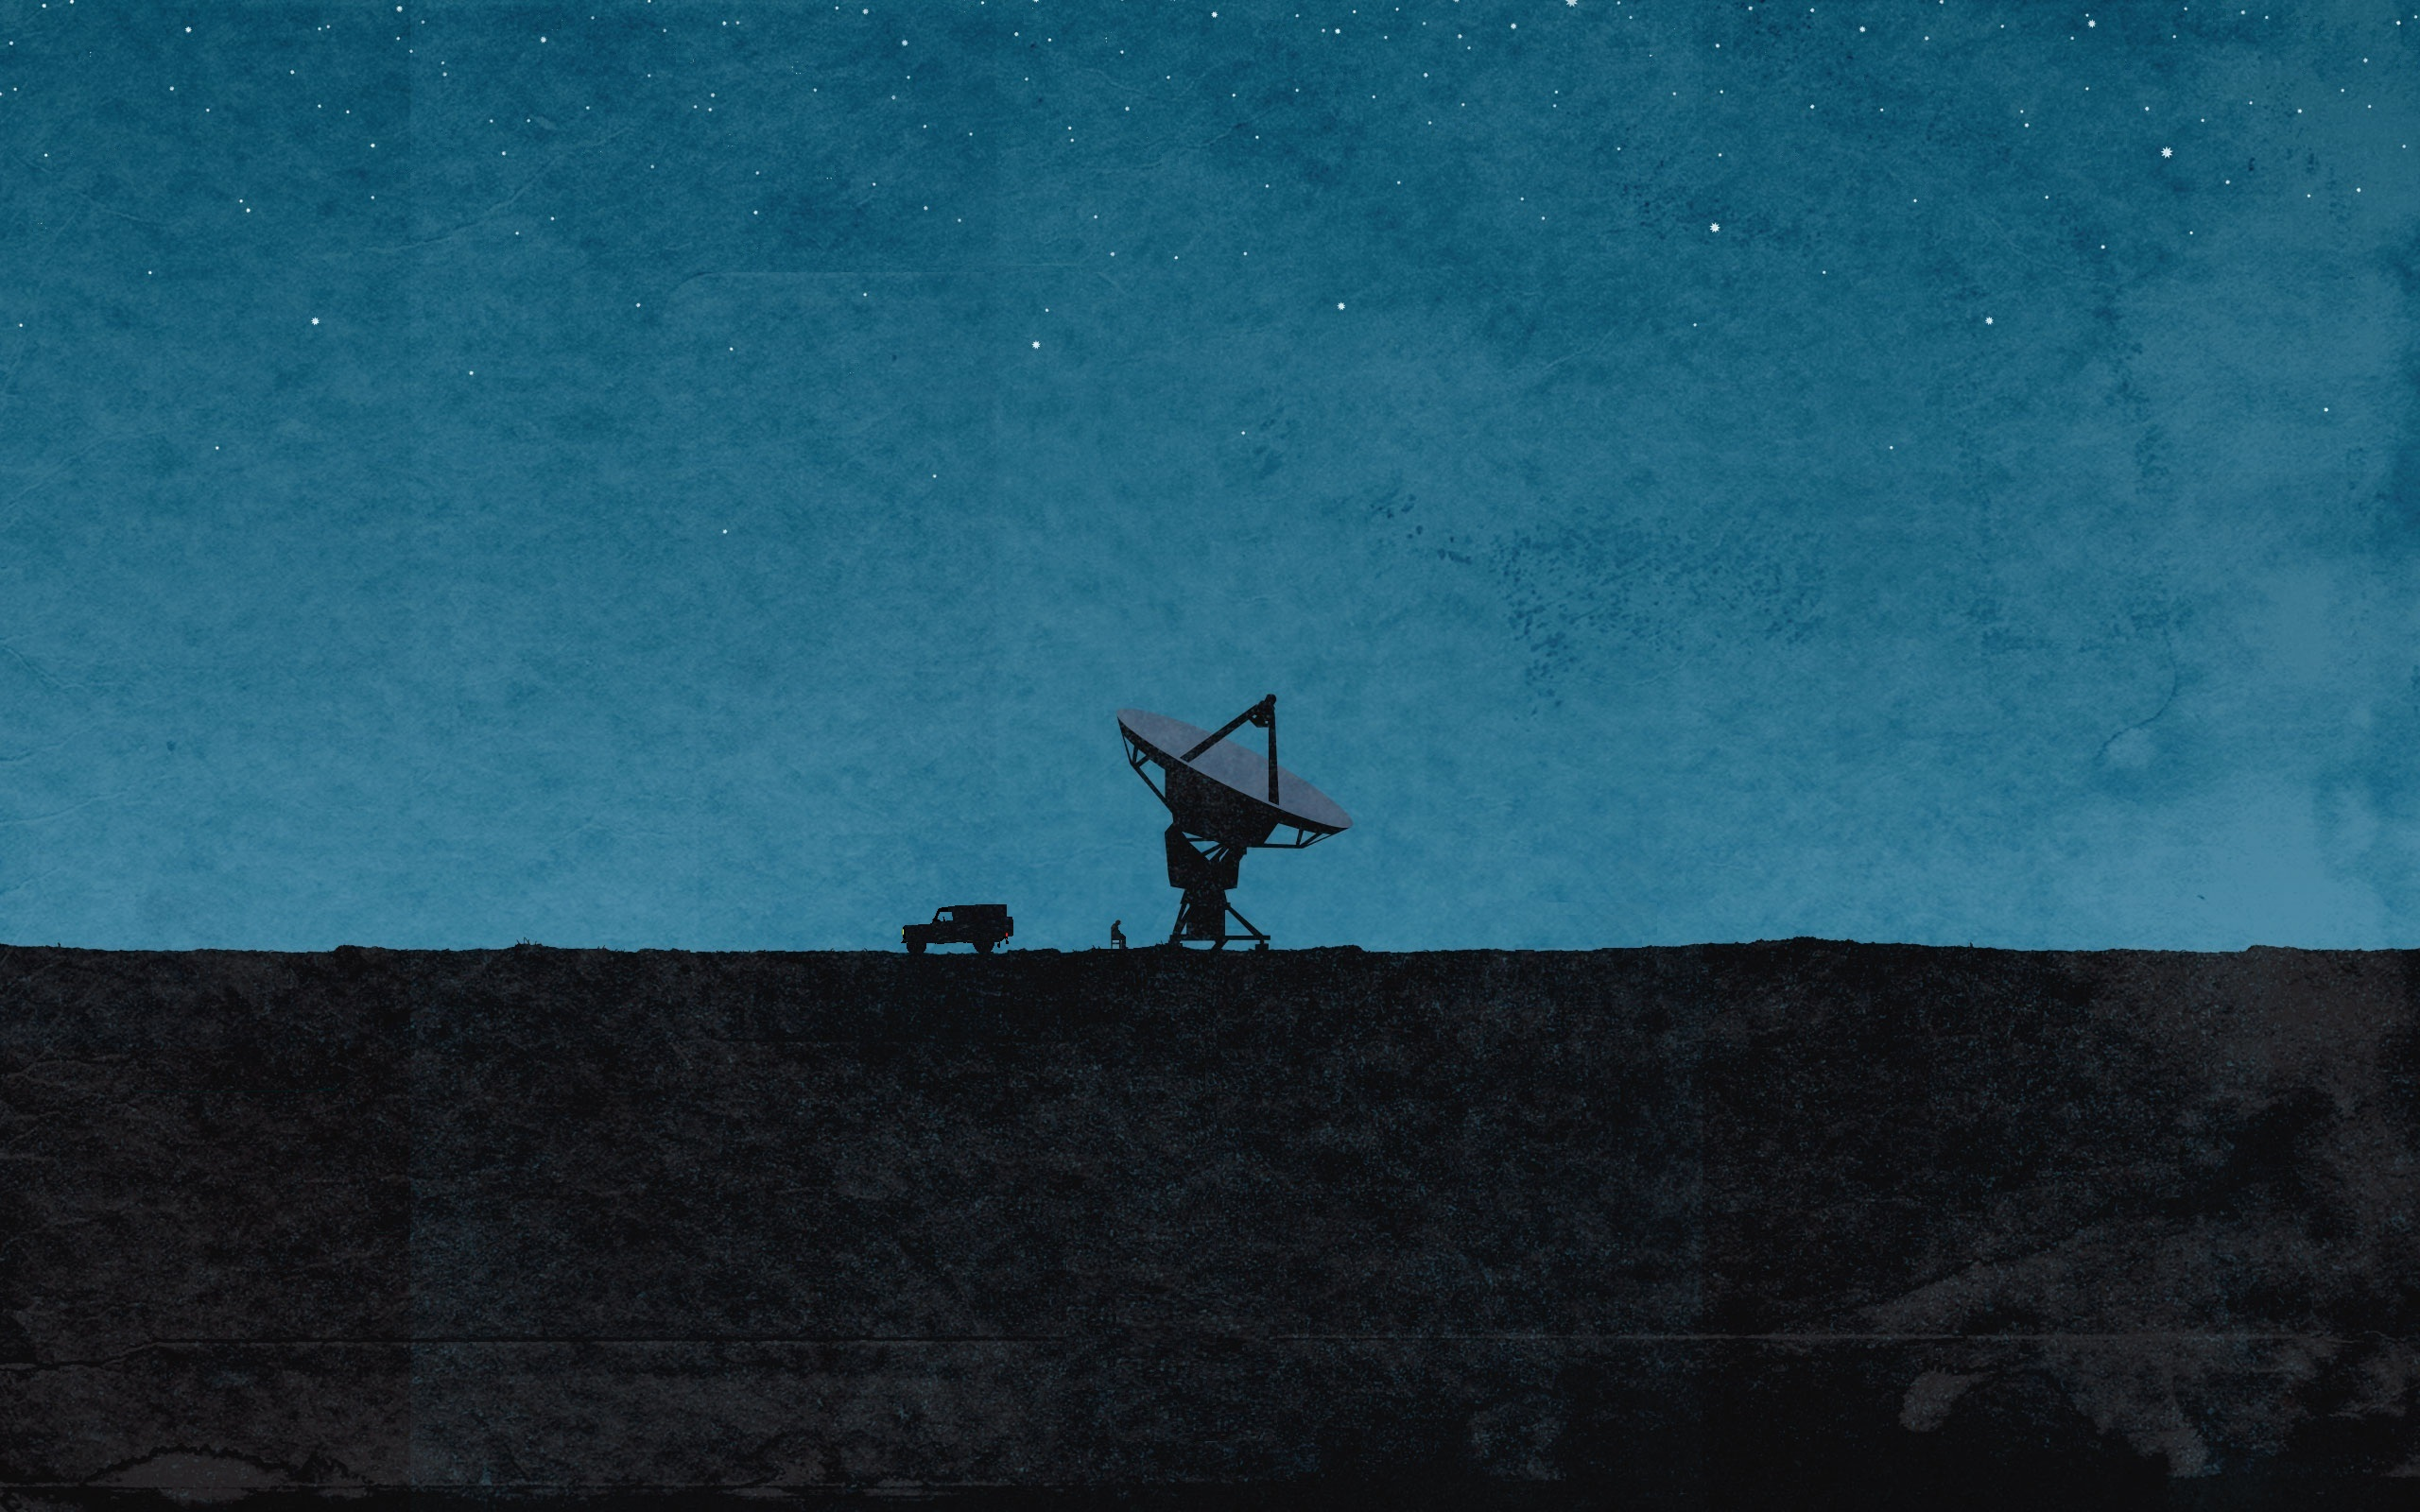
\includegraphics[width=1.0\textwidth]{./images/image.jpg}
    \caption{Awesome Image}
    \label{fig:awesome_image}
\end{figure}

lkasjdflkj asldkjf lasjkdflkadsjf ladksjflkjslkdjf    dslfjklaks df a sdfjaldsfj  ladksjf lkjlakjsd f asdf aljsdflkjasldfjalsdfj l adskjflj d f dslkfjalksdjf sd fljsdfkjsld f

\emph{dieser text ist kursiv}

asdfasdfasdfasdlkvalrkgjval  asdkfj  sldkfjlsdjfa adaher is kes ji lkaskdj ladskj a ldksfjll aldkfj lkj afsdlfkjl alsdkf jaldskfj la sdflaldsflas df sadfl sf

\texttt{das hier ist monotype}

% TODO: reformat chapter style with package titlesec
%\titleformat{\section}
%{\filcenter\normalfont\Large\bfseries}
%{\chaptertitlename~\thechapter} {0.5em} {}


\chapter{Überblick/Einführung}
	\section{Arten von Virtualisierungen}
	\section{Einordnung Docker}
\chapter{Ziel der Arbeit/Forschungsfrage}
\chapter{Security aus Linux Kernel-Features}
	\section{Isolierung}
		\subsection{\texttt{namespaces}}
			\subsubsection{\texttt{user namespaces}}
		\subsection{\texttt{capabilities}}
			\subsubsection{Beispiele, \texttt{/proc}-Verzeichnis, (Un-)Mounten des Host-Filesystems}
		\subsection{Mandatory Access Control (MAC)}
			\subsubsection{Beispiel SELinux}
	\section{Ressourcenverwaltung}
		\subsection{\texttt{cgroups}}
	\section{Docker im Vergleich zu anderen Containerlösungen}
\chapter{Security im Docker-Ökosystem}
  \section{Docker Images und Repositories}
		\subsection{neues Signierungs-Feature}
	\section{Docker Daemon}
		\subsection{REST-API}
		\subsection{Support von Zertifikaten}
	\section{Docker Cache}
	\section{\texttt{privileged} Container}
	\section{Networking}
		\subsection{\texttt{bridge} Netzwerk}
		\subsection{\texttt{overlay} Netzwerk}
		\subsection{DNS}
		\subsection{Portmapping}
	\section{Daten-Container}
	\section{Docker mit VMs}
	\section{Tools rund um Docker}
		\subsection{Docker Swarm}
		\subsection{Docker Compose}
		\subsection{Nautilus Project}
		\subsection{Vagrant}
		\subsection{Kubernetes}
\chapter{Docker in Unternehmen/Clound-Infrastrukturen}
% HIER: welche Security-Features uebernimmt die Cloud, welche muss Docker
% geaehrleisten. Was bieten MS Azure/Amazon's AWS/etc fuer Mechanismen an?
% Welche Moeglichkeiten zur sicheren Docker-Integration bieten diese?
% Wortlaut Patrick: Wie funktionierts bei Azure, wie funktionierts wenn man es
% selbst implementiert.
\chapter{Fazit}

%\subsection{Subsektion blabla}
%\subsubsection{Subsubsektion blablabla}
%\paragraph{Paragraph soundso}
%\subparagraph{SubParagraph soundso}



% Anhang
\appendix

% Bibliography
\bibliographystyle{plain}
\bibliography{test} % specify name of bibfile

\end{document}
